\chapter{Revisão bibliográfica}\label{chp:revisao}
\section{Etinilestradiol}

O \Sigla{etinilestradiol}{EE} é um derivado sintético do estradiol, um tipo de estrogênio. Ele é comumente utilizado em combinação com outros hormônios como contraceptivo, no tratamento de certos distúrbios ginecológicos, alguns cânceres dependentes de hormônios (como câncer de próstata e câncer de mama) e sintomas da menopausa. Como contraceptivo, está geralmente disponível em baixas concentrações, pois possui alguns efeitos colaterais como ganho de peso, dor de cabeça, náuseas e inchaço. Assim, é crucial que a formulação seja estável e mantenha sua eficácia ao longo do tempo (Simu et al. 2022).

Os estrogênios são hormônios produzidos naturalmente pelo corpo humano em diversas formas, sendo elas estradiol, estrona, estriol e seus conjugados. Sua ação se dá através de dois mecanismos, sendo um genômico e outro não genômico. No caso do mecanismo genômico, ocorre a interação com proteínas específicas localizadas no núcleo das células, os chamados receptores de estrogênio, ER$\alpha$ e ER$\beta$. Essa interação pode modificar alguns genes, ativando ou desativando a produção de certas proteínas específicas, necessárias para diversas funções do organismo. Já no mecanismo não genômico, a interação se dá com diferentes receptores localizados na superfície das células e acoplados a moléculas chamadas proteínas G. Essa interação dispara uma cadeia de reações dentro das células, alterando rapidamente seu comportamento sem que haja modificação dos genes. Dessa forma, o estrogênio produz efeitos no corpo tanto no curto quanto no longo prazo (Kuhl 2005).

O estradiol 17$\beta$, cuja fórmula estrutural pode ser observada na \Figura{fig:structure} \Subfigura{fig:estradiol}, é o mais importante estrogênio endógeno nos seres humanos e o mais potente. Ele possui papel essencial na reprodução e também está envolvido em vários processos metabólicos, afetando o organismo como um todo. O etinilestradiol (17$\alpha$-etinilestradiol ou EE) é um derivado sintético desse estrogênio que possui um grupo etinil na posição 17$\alpha$ sendo sua fórmula estrutural representada na \Figura{fig:structure} \Subfigura{fig:etinilestradiol}. Essa diferença na estrutura protege o grupo hidroxila localizado na posição 17$\beta$ da degradação por oxidação (Kuhl 2005). Como consequência, o EE é caracterizado por maiores atividade farmacológica, biodisponibilidade, resistência ao metabolismo e efeitos mais fortes em certas partes do corpo (Simu et. al. 2022).

\begin{figure}[!htb]
    \begin{center}
    \subfloat[Estradiol 17$\beta$]{%
        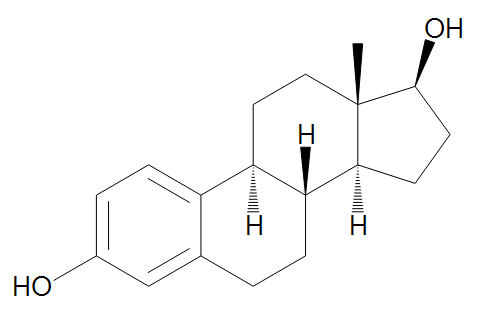
\includegraphics[width=0.48\textwidth]{figuras/estradiol17b.png}
        \label{fig:estradiol}
    }\hfill
    \subfloat[Etinilestradiol]{%
        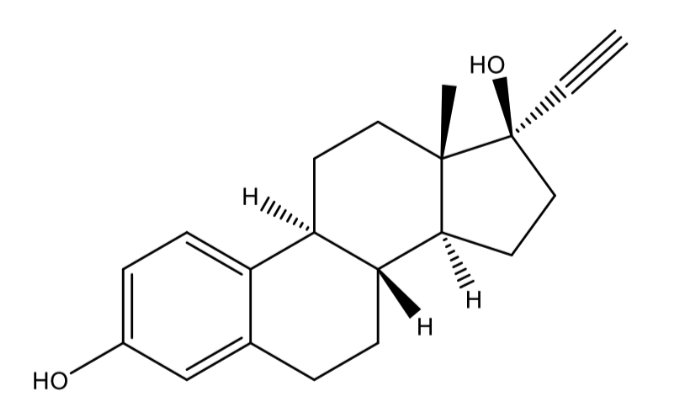
\includegraphics[width=0.48\textwidth]{figuras/etinilestradiol.png}
        \label{fig:etinilestradiol}
        }\par
    \caption[Estradiol 17$\beta$ e etinilestradiol.]{Fórmulas estruturais do estradiol 17$\beta$ \Subfigura{fig:estradiol} e do etinilestradiol \Subfigura{fig:etinilestradiol}.}
    \label{fig:structure}
    \end{center}
\end{figure}

No mercado farmacêutico em todo o mundo, existem diversas fórmulas contendo o etinilestradiol, além de uma variedade de possibilidades de administração, como oral, transdermal e vaginal. A via oral de administração de hormônios contraceptivos é muito bem estabelecida e se trata de comprimidos de administração diária. A via transdermal é realizada através de adesivos aplicados sobre a pele e trocados semanalmente, enquanto a vaginal é feita por um anel de silicone inserido uma vez por mês (Heuvel et al. 2005).

Um grande desafio na indústria farmacêutica diz respeito às matrizes de liberação de medicamentos e sua consistência a longo prazo. Certos fármacos perdem eficácia ao longo do tempo, com sua concentração caindo abaixo do mínimo necessário para a eficácia do tratamento, ou, pelo contrário, acabam ultrapassando a concentração tóxica mínima e produzindo assim efeitos adversos. Por isso, é importante investigar o uso de modelos matemáticos a fim de aprimorar a compreensão da liberação controlada de medicamentos (Simon 2004). A construção desses modelos deve levar em consideração as dinâmicas de absorção do meio, e por isso requer o conhecimento de fenômenos de transporte e transferência de massa (Simon 2007).

\section{Matrizes}

A Organização Mundial da Saúde (OMS) considera o acesso ao planejamento familiar seguro essencial para a promoção da autonomia das mulheres e para a igualdade de gênero. Um elemento citado como fundamental para a qualidade do planejamento familiar é o acesso à escolha entre uma variedade de métodos contraceptivos, bem como à informação para realizar a escolha baseada na eficácia, segurança e benefícios de cada um. Dentre as categorias de escolha recomendadas, estão os \Sigla{contraceptivos hormonais combinados}{CHCs}: as pílulas anticoncepcionais, os adesivos contraceptivos e os anéis vaginais contraceptivos (World Health Organization, 2016).

No mercado mundial, existem diversas fórmulas contendo o etinilestradiol, seja como princípio ativo único ou associado a outro componente, como dienogeste e levonorgestrel, para administração oral (pílula anticoncepcional),  vaginal (anel) ou transdérmica (adesivo). Dependendo da rota de administração, a quantidade de EE na formulação pode variar (Simu et. al., 2022). Sabe-se que os estrogênios possuem efeitos colaterais como dores nos seios, dor de cabeça, retenção de fluidos e náusea, além de trazerem riscos de tromboembolismo (Stanczyk et al., 2013). Contudo, comparando os CHCs, é possível observar entre eles diferenças na exposição ao EE e na ocorrência dos efeitos adversos (Heuvel et al. 2005).

\subsection{Contraceptivos orais combinados}

Os \Sigla{contraceptivos orais combinados}{COCs} têm ajudado milhões de mulheres em todo o mundo a evitar gravidezes não desejadas desde a sua introdução no mercado, nos anos 1960, e seguem hoje sendo a forma de controle de natalidade mais popular. A maior parte dos COCs do passado e presente contém etinilestradiol como componente estrogênico. Para administração oral, o etinilestradiol é usado em uma forma microcristalina a fim de maximizar a superfície de contato, o que possibilita absorção mais eficaz e aumenta sua biodisponibilidade. A formulação do COC pode conter de menos de 20 \textmu g a 30 \textmu g de EE (Kuhl, 2005; Stanczyk et al., 2013). Na \Figura{fig:pills} abaixo, estão dois exemplos de fórmulas comerciais contendo o etinilestradiol em diferentes quantidades.

\begin{figure}[!htb]
    \begin{center}
    \subfloat[Tâmisa\textsuperscript{\textregistered}]{%
        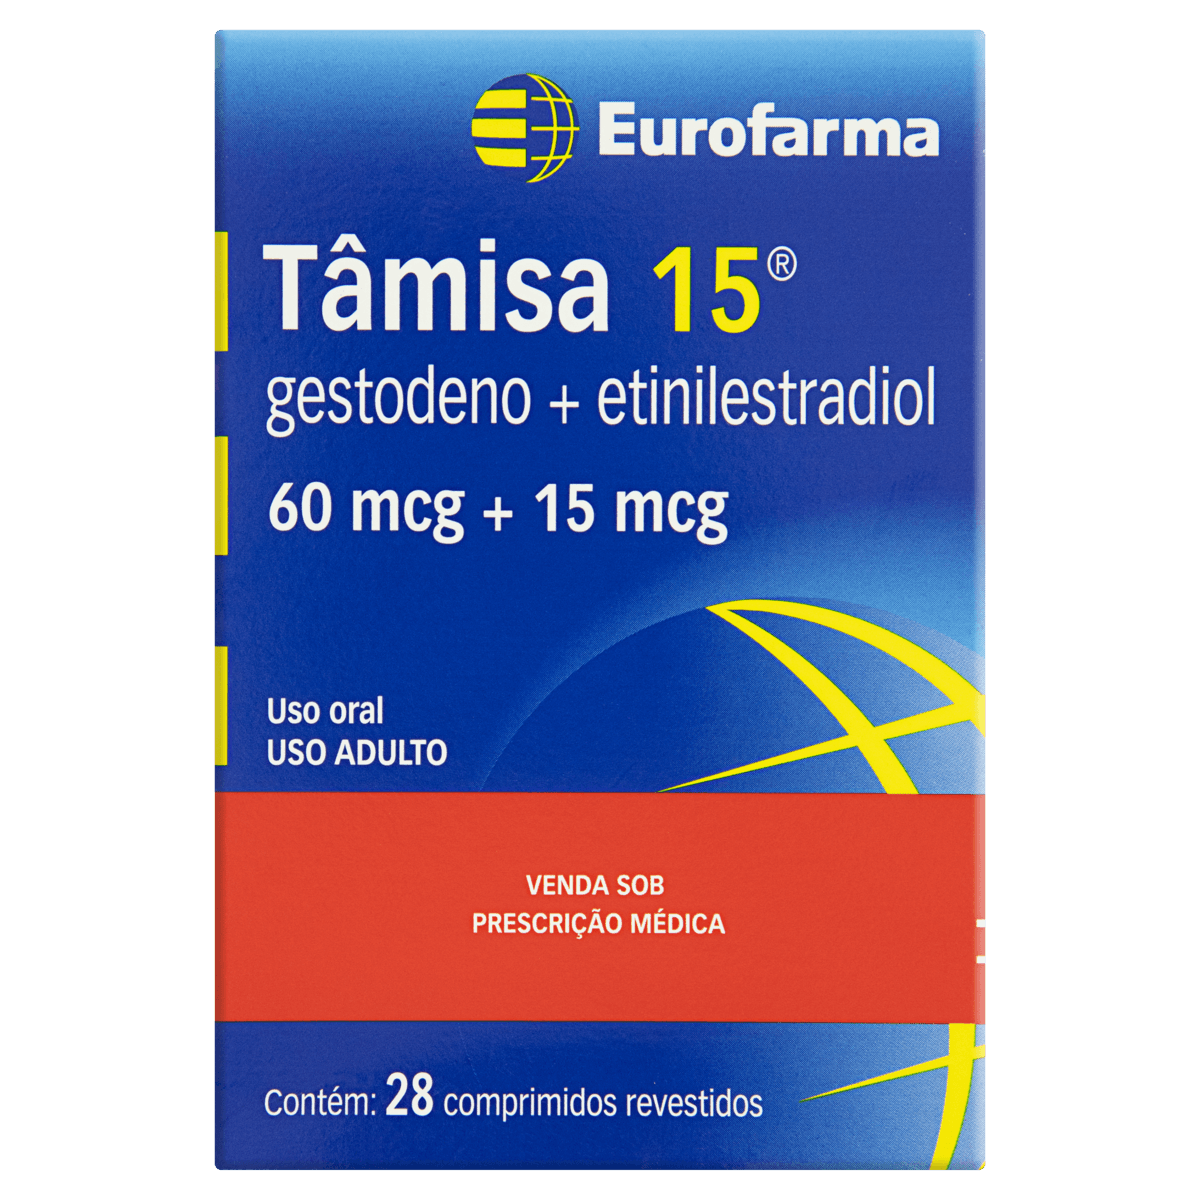
\includegraphics[width=0.28\textwidth]{figuras/Tamisa.png}
        \label{fig:tamisa}
    }\hfill
    \subfloat[Microgynon\textsuperscript{\textregistered}]{%
        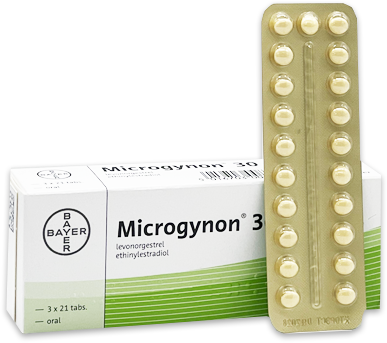
\includegraphics[width=0.28\textwidth]{figuras/Microgynon-Tablets-Side.png}
        \label{fig:microgynon}
        }\par
    \caption[COCs comerciais]{Os COCs Tâmisa\textsuperscript{\textregistered} \Subfigura{fig:tamisa} e Microgynon\textsuperscript{\textregistered}  \Subfigura{fig:microgynon} são exemplos de fórmulas comerciais contendo o etinilestradiol (e-Surgery, 2024; Santa Lúcia Drogarias, 2024).}
    \label{fig:pills}
    \end{center}
\end{figure}

O etinilestradiol é rapidamente absorvido após a administração oral de doses terapêuticas, sendo o pico de concentração plasmática atingido de 1 a 2 horas após a ingestão (Stanczyk et al., 2013). A dosagem diária da pílula produz picos e vales na concentração de EE no sangue ao longo do tempo (Heuvel et al. 2005). A administração oral possui como vantagens o fato de ser fácil e conveniente, não invasiva e rapidamente reversível. Por outro lado, devido à alta atividade metabólica que ocorre no sistema digestivo, são necessárias concentrações mais elevadas do princípio ativo do que em outras matrizes, causando também maior impacto no fígado (Kuhl, 2005).

A maior preocupação existente sobre os COCs diz respeito a seus efeitos colaterais indesejados, principalmente coágulos sanguíneos, ataques cardíacos, AVCs, ganho de peso e perda de libido (Stanczyk et al., 2013). Além disso, sua eficácia depende da ingestão diária correta e consistente, o que acarreta em uma taxa anual de falha de 8\% no uso típico (Lubianca, 2016). 

De acordo com o Ministério da Saúde (s.d.), o Programa Saúde da Mulher disponibiliza comprimidos contendo etinilestradiol para distribuir gratuitamente à população, sendo também parte do Programa Farmácia Popular. Já nas farmácias, o valor de uma caixa de 21 comprimidos pode variar entre R\$18 e R\$96, a depender da composição e do laboratório, segundo dados de Preço Máximo ao Consumidor (PMC) obtidos das Listas de Preços de Medicamentos da ANVISA (2024).

\subsection{Adesivo transdérmico}

O fator do esquecimento e o ônus da ingestão diária de medicamento podem ser contornados pela alternativa da administração de fármacos através da pele, levando o princípio ativo diretamente à circulação sanguínea. Ao evitar a passagem pelo trato gastrointestinal, evita-se também o chamado metabolismo de primeira passagem, fenômeno no qual o fármaco passa pelo fígado antes de entrar na circulação geral, tendo sua concentração reduzida (Scheindlin, 2004; Lin et. al., 2010). Os adesivos transdérmicos foram desenvolvidos com a finalidade de aumentar a adesão e conforto dos pacientes, além de aumentar a biodisponibilidade do fármaco no organismo e possibilitar administração continuada de fármacos com meia-vida curta (Saroha, 2016).

Os adesivos transdérmicos podem ser de dois tipos: matriz ou reservatório. No sistema adesivo em reservatório, o princípio ativo fica em um reservatório líquido, em uma solução de álcool. Já no sistema em matriz, utilizado nos contraceptivos, as moléculas ficam distribuídas uniformemente ao longo de uma matriz polimérica, sendo a difusão do estrogênio para a pele facilitada por alguma substância como um ácido graxo ou etanol. A camada externa é geralmente de poliéster, \Sigla{copolímero etileno acetato de vinila}{EVA} ou poliuretano, enquanto o adesivo é um polímero de acrilato. A taxa de difusão no sistema matricial é mais constante em comparação ao sistema reservatório (Scheindlin, 2004; Kuhl, 2005). A \Figura{fig:patch} mostra uma esquematização das camadas do adesivo do tipo matriz.

\begin{figure}[!htb]
    \centering
        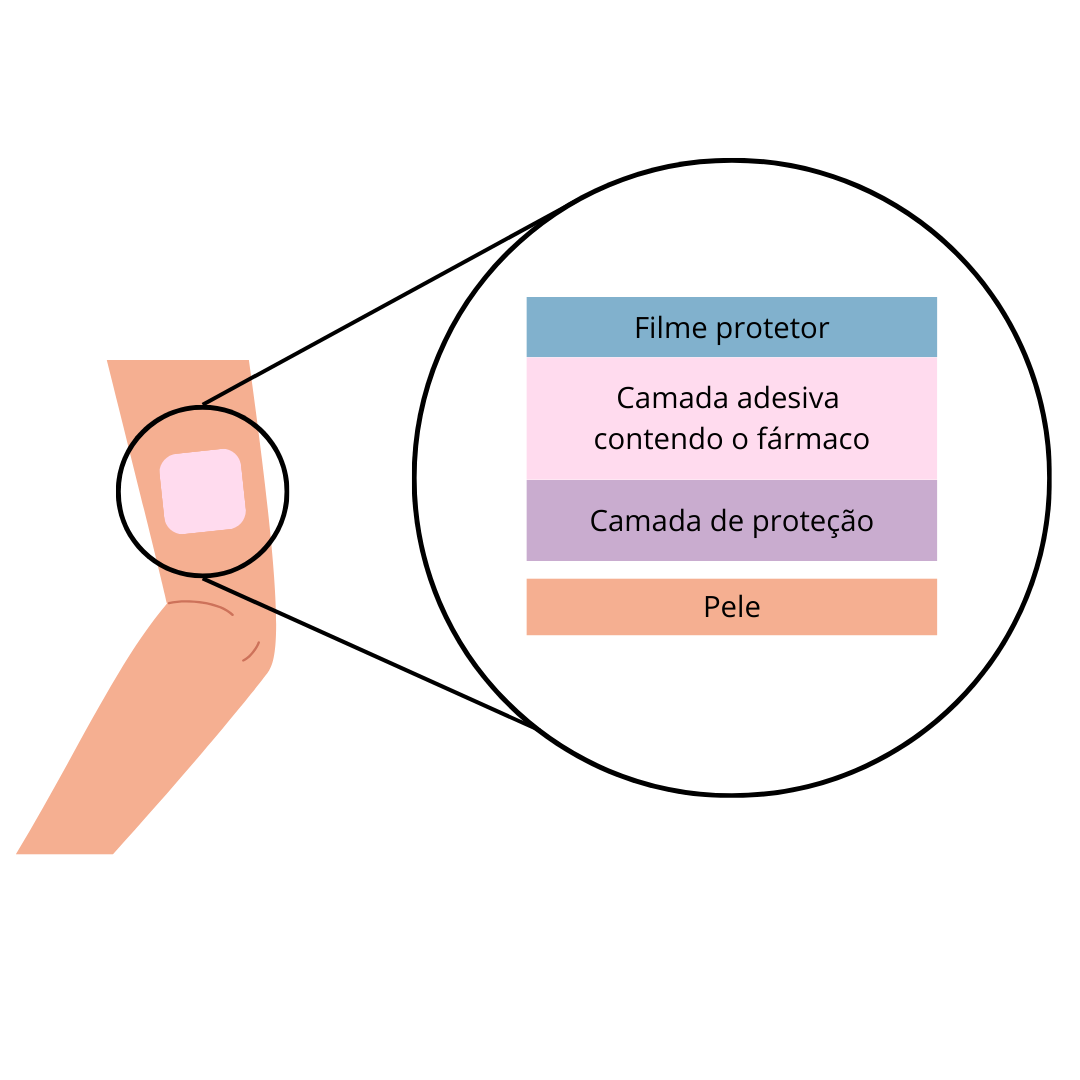
\includegraphics[width=0.48\textwidth]{figuras/adesivo.png}
        \caption[Camadas do adesivo transdérmico do tipo matriz]{Camadas do adesivo transdérmico do tipo matriz. A camada de proteção é removida antes da aplicação (adaptado de Scheindlin, 2004).}
    \label{fig:patch}
\end{figure}

A eficácia da administração de fármacos pela via transdérmica depende da permeabilidade do fármaco em questão na pele. O fluxo é mantido devido a um gradiente de concentração entre o local da aplicação e os capilares sanguíneos. Os pontos negativos da utilização dos adesivos transdérmicos são a dificuldade de ultrapassar a barreira da pele e a possibilidade de reações alérgicas na paciente (Saroha, 2016). Dependendo do tempo que ficam com o adesivo no mesmo local, entre 50 e 60\% das pacientes apresentam vermelhidão de leve a moderada, podendo restar resíduos do adesivo na pele após a retirada (Kuhl, 2005).

Os adesivos contraceptivos são contraceptivos hormonais combinados de aplicação tópica semanal, devendo assim ser aplicados três vezes ao mês. As composições podem variar, podendo chegar a conter 750 \textmu g de etinilestradiol por adesivo (Devineni et. al., 2007). Em geral, os adesivos são projetados para fornecer cerca de 20 \textmu g de EE por dia (Heuvel et al. 2005).

Um estudo de Heuvel et al. (2005) comparando os efeitos da pílula, anel vaginal e adesivo transdérmico contendo etinilestradiol em grupos de mulheres utilizando cada um desses CHCs demonstrou que, apesar de o adesivo ser projetado para fornecer uma dose diária baixa de EE, a exposição ao EE nesse grupo foi a mais alta entre os três, bem como a incidência de efeitos adversos relacionados ao estrogênio. Segundo o estudo, isso pode indicar uma maior eficiência do adesivo em termos de entrega de EE ao corpo, podendo ser utilizado, por exemplo, pelas pacientes que possuem menor sensibilidade aos efeitos colaterais e precisam de uma maior garantia de absorção. 

O adesivo contraceptivo não está incluso entre os medicamentos de distribuição gratuita pelo governo e o preço de uma caixa contendo três adesivos, quantidade suficiente para um mês de contracepção, pode variar entre R\$50 e R\$130 (UOL, 2021; ANVISA, 2024).

\subsection{Anel vaginal}

Os anéis vaginais contraceptivos oferecem, assim como os adesivos transdérmicos, a vantagem de evitar o metabolismo hepático de primeira passagem, oferecendo uso continuado fácil e alta biodisponibilidade de hormônios. Tratam-se de anéis circulares de material polimérico, como o silicone, cuja utilização se dá através da inserção no canal vaginal, onde o dispositivo deve permanecer por 21 dias do mês. O anel vaginal comercial mais conhecido é o NuvaRing{\textregistered}, um anel circular de EVA com estearato de magnésio, que possui 54 mm de diâmetro e 4 mm de espessura, e tem como componente estrogênico o etinilestradiol. Diariamente, o NuvaRing libera para a corrente sanguínea cerca de 15 \textmu g de EE (Barnhart et. al., 2005; Heuvel et al., 2005). A \Figura{fig:nuvaring} mostra o NuvaRing. 

\begin{figure}[!htb]
    \centering
        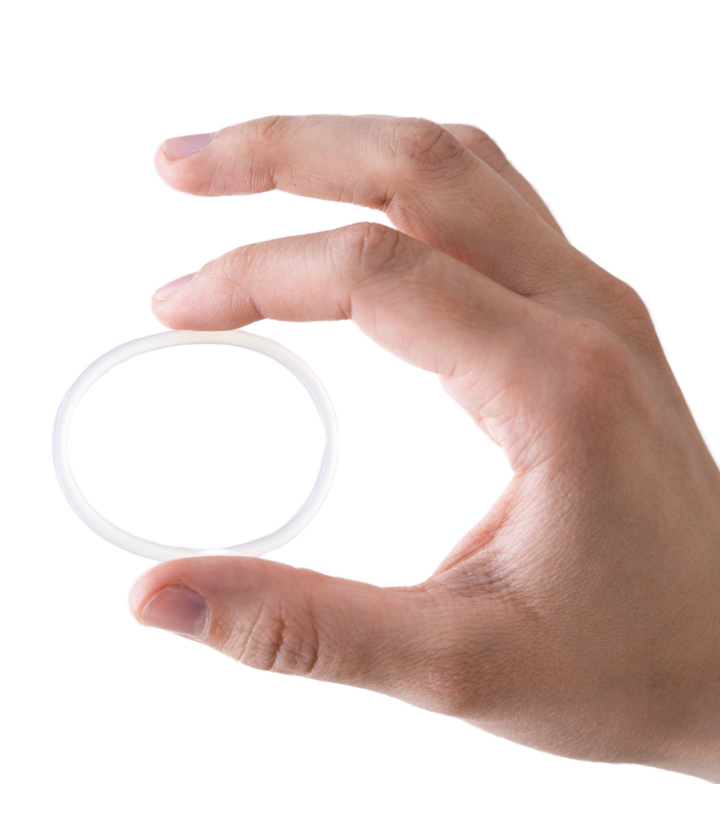
\includegraphics[width=0.38\textwidth]{figuras/nuvaring.png}
        \caption[Anel vaginal]{O anel vaginal contraceptivo NuvaRing{\textregistered} (NuvaRing, 2024).}
    \label{fig:nuvaring}
\end{figure}

O conceito dos anéis vaginais contraceptivos é baseado em dois princípios: a capacidade dos hormônios esteróides, como os estrogênios, de  difundirem lentamente a uma taxa constante através de polímeros biocompatíveis e a capacidade do epitélio do canal vaginal de absorver rapidamente esses hormônios (Faundes et. al, 2004). Por causa disso, a concentração sanguínea de etinilestradiol após a administração vaginal pode ser de 10 a 20 vezes maior do que após a administração oral da mesma dose (Kuhl, 2005).

Dessa forma, a administração pela via vaginal permite uma dosagem baixa, estável e contínua, resultando em uma concentração estável de hormônio no sangue. Isso é benéfico porque minimiza a exposição ao EE, diminuindo a probabilidade da incidência de efeitos colaterais relacionados ao estrogênio (Heuvel et al. 2005). Contudo, a maioria dos dispositivos possui um efeito de liberação inicial rápida antes de atingir um estado estacionário na taxa de liberação, o que provavelmente se deve ao acúmulo de hormônios na superfície do anel durante o armazenamento (Faundes, 2004).

A eficácia contraceptiva do anel vaginal é considerada boa, sendo similar ou um pouco melhor do que a obtida com contraceptivos orais. Ele é fácil de usar, pois necessita de ação por parte da paciente em apenas dois dias por mês, sendo um dia para inserção, no início do ciclo, e outro para retirada, três semanas depois. A conveniência, facilidade e eficácia são as vantagens mais citadas pelas usuárias do anel. Como pontos contrários, estão a inserção no canal vaginal, que pode ser desconfortável ou encontrar resistências culturais em algumas partes do mundo,  além de causar maior probabilidade de sintomas e lesões vaginais em comparação com a utilização dos COCs (Faundes, 2004). 

O estudo comparativo realizado por Heuvel et al. (2005) indicou que o grupo que utilizou o NuvaRing foi o que apresentou a menor variação nos níveis de EE no sangue, em média 3,4 vezes menor do que das pacientes que usaram o adesivo transdérmico e aproximadamente duas vezes menor do que daquelas que usaram o COC. Essas diferenças na farmacocinética do EE entre os diferentes métodos podem ter implicações importantes na escolha do método contraceptivo baseado no perfil de risco e benefício individual de cada paciente.  Os resultados obtidos por esse estudo indicam que a administração vaginal de etinilestradiol com o NuvaRing proporciona uma dosagem muito menor, mais estável e mais precisa do que as vias transdérmica e oral, resultando em uma baixa exposição ao EE e podendo ser indicado a pacientes que possuem sensibilidade aos efeitos do estrogênio. O anel vaginal não está entre os contraceptivos disponíveis gratuitamente pelos programas do governo, e seu valor pode variar entre R\$94 e R\$124 para 1 mês de contracepção (ANVISA, 2024).

\section{Modelagem matemática da liberação de fármacos}

\subsection{Difusão fickiana em membranas orgânicas}

De acordo com a segunda lei da termodinâmica, haverá fluxo de matéria de uma região de maior a outra de menor concentração de uma determinada espécie química, sendo essa espécie denominada soluto. Assim, define-se a transferência de massa como o fenômeno ocasionado pela diferença de concentração, maior para menor, de um determinado soluto em um certo meio. Quando há ação substancial da concentração do soluto no espaço considerado e o transporte ocorre em nível molecular, de forma que a força motriz é o gradiente de concentração, esse fenômeno é conhecido como difusão. Na difusão, a resistência ao transporte está associada somente à interação soluto-meio (Cremasco, 2015).

A difusão pode ocorrer através de membranas, que atuam como barreiras ao transporte, separando dois fluidos e devendo ser vencidas pelo soluto. As membranas podem ser compostas por materiais inorgânicos ou orgânicos, apresentar poros ou não. Na indústria, são utilizadas em diversos processos de separação, tais como adsorção, absorção, secagem, combustão, cristalização, extração, lixiviação e destilação. As membranas feitas de materiais orgânicos são normalmente classificadas como membranas densas, e a descrição da difusão mássica através delas dá-se em virtude das características dos polímeros que as constituem. Esse tipo de membrana é utilizado, por exemplo, na ultrafiltração (Cremasco, 2015; Cremasco, 2019).

As membranas orgânicas, utilizadas normalmente na indústria química e correlatas, são chamadas de membranas isotrópicas densas. Elas são isentas de poros, e o fenômeno da difusão é, portanto, determinado pela interação soluto–polímero. A difusão de um soluto em um polímero ocorre por um processo de estado ativado, via saltos energéticos, ocupando vazios na estrutura polimérica. Tais sítios vagos são fruto do entrelaçamento dos segmentos da cadeia macromolecular, e fazem com que o material se comporte como uma matriz porosa, apesar de não possuir poros fixos. Admitindo que o diâmetro dos poros da estrutura seja muito maior do que o diâmetro de difusão do soluto, e desde que não ocorra variação do volume da matriz, a difusão do soluto em regime permanente será regida pela Primeira Lei de Fick,

\begin{equation}
J_{A,z} = -D_{AB} \frac{dC_A}{dz}
\end{equation}

\noindent sendo $J_{A,z}$ o fluxo de difusão molar do soluto $A$ na direção $z$, $C_A$ a concentração molar do soluto e $D_{AB}$ o coeficiente binário de difusão do soluto A no meio B (Cremasco, 2015; Cremasco, 2019).

\subsection{Difusão na absorção percutânea de fármacos}

A absorção percutânea de fármacos envolve a penetração de um princípio ativo através da pele, sua absorção pelos capilares e distribuição na circulação sistêmica. A Segunda Lei de Fick é comumente utilizada para modelar esse processo. No entanto, diversos fatores importantes precisam ser considerados, como a escolha da membrana, o projeto do sistema de liberação, que simula a aplicação do fármaco, e o tempo de exposição. Além disso, é igualmente essencial contar com uma descrição matemática, que permita prever o comportamento do fármaco com precisão (Simon, 2005).

A Segunda Lei de Fick é representada por uma \Sigla{equação diferencial parcial}{EDP} linear e de segunda ordem que descreve a distribuição de concentração do soluto no tempo e no espaço, para casos em que o regime é transiente e o coeficiente de difusão não depende da concentração do soluto (Cremasco, 2019). Ela é escrita na forma:

\begin{equation}
\frac{\partial C_A}{\partial t} = D_{AB} \frac{\partial^2 C_A}{\partial z^2}
\end{equation}

\noindent e tem sido utilizada na literatura para descrever permeação cutânea de fármacos em que o estado estacionário é atingido após determinado período. Nessa modelagem, tanto a matriz do fármaco quanto a pele são descritas como membranas orgânicas fickianas (Kubota et. al, 2002; Simon, 2005). Kubota et. al (2002) e Simon (2007) utilizaram essa modelagem em seus trabalhos, representando os sistemas como mostrado na \Figura{fig:modelo_adesivo} em que $C_1$ representa a concentração de medicamento na matriz e $C_2$, na pele.

\begin{figure}[!htb]
    \centering
        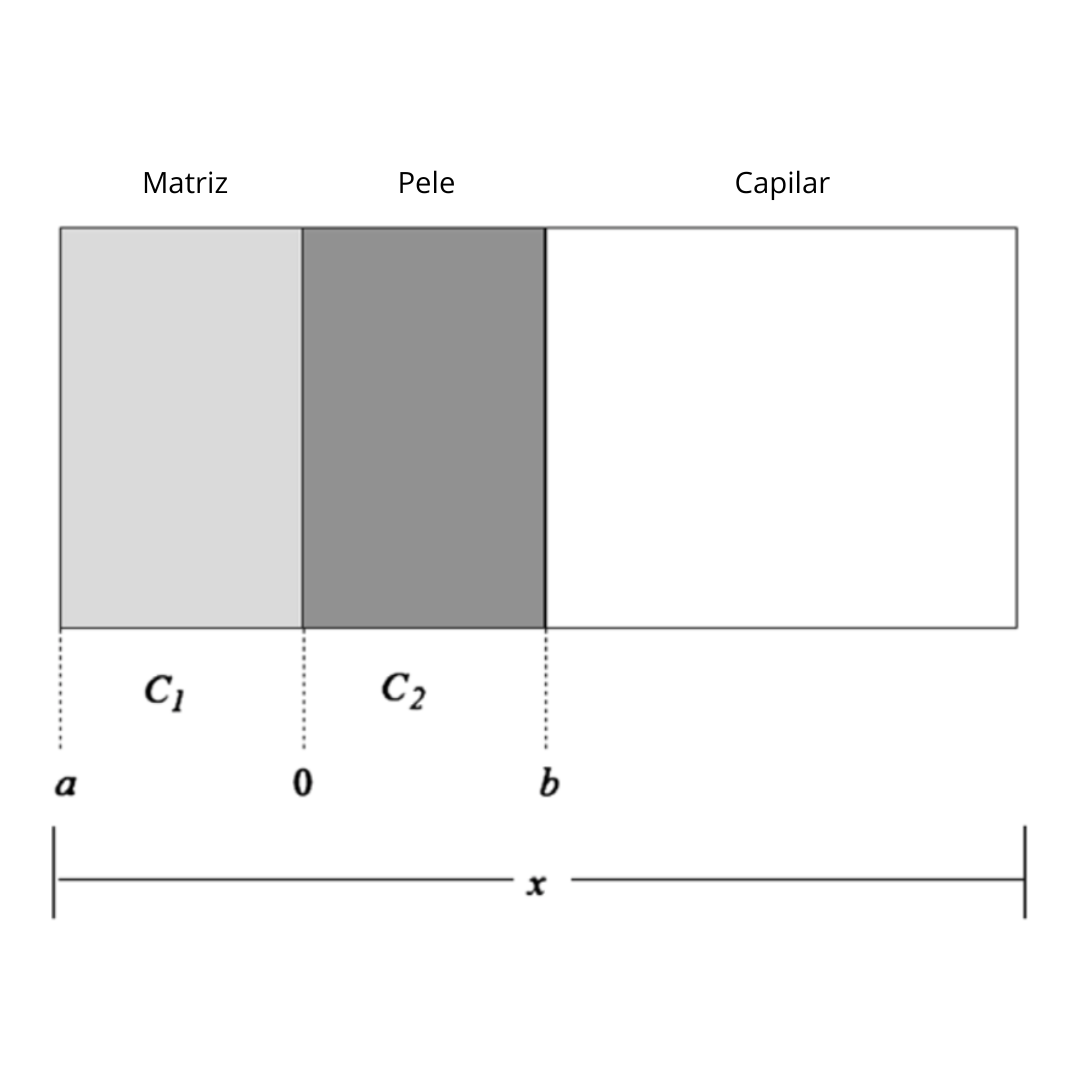
\includegraphics[width=0.48\textwidth]{figuras/modelo_adesivo.png}
        \caption[Representação esquemática de absorção percutânea]{Representação esquemática de absorção percutânea de fármaco (adaptado de Simon, 2007). }
    \label{fig:modelo_adesivo}
\end{figure}

Segundo esse modelo, temos:

\begin{equation}
\frac{\partial C_1}{\partial t} = D_1 \frac{\partial^2 C_1}{\partial x^2}, \quad a < x < 0, \quad 0 < t \leq T
\end{equation}

\begin{equation}
\frac{\partial C_2}{\partial t} = D_2 \frac{\partial^2 C_2}{\partial x^2}, \quad 0 < x < b, \quad 0 < t \leq T
\end{equation}

\noindent em que $D_1$ e $D_2$ são os coeficientes de difusão na matriz e na pele, e $a$ e $b$ são as espessuras da matriz e da pele, respectivamente. $T$ é o período de aplicação.

Simon (2007) ainda definiu as seguintes condições iniciais:

\begin{equation}
C_1[x,0] = C_{10}, \quad a < x < 0
\end{equation}

\begin{equation}
C_2[x,0] = C_{20}, \quad 0 < x < b
\end{equation}

\noindent e as condições de contorno:

\begin{equation}
\frac{\partial C_1(a,t)}{\partial x} = 0, \quad 0 < t \leq T
\end{equation}

\begin{equation}
\frac{D_1\partial C_1[0,t]}{\partial x} = \frac{D_2\partial C_2[0,t]}{\partial x}, \quad 0 < t \leq T
\end{equation}

\begin{equation}
K_m C_1[0,t] = C_2[0,t], \quad 0 < t \leq T
\end{equation}

\begin{equation}
- \frac{D_2\partial C_2[b,t]}{\partial x} = K_{cl}C_2[b,t], \quad 0 < t \leq T
\end{equation}

\noindent em que $K_m$ é o coeficiente de partição matriz-pele e $K_{cl}$ é chamado de \textit{clearance} (depuração) por unidade de área do medicamento por unidade de excesso de concentração em $x = b$. Na Eq. (2.7), garante-se que não ocorre transferência de massa entre a matriz e o ambiente; a Eq. (2.8) representa a continuidade do fluxo através da interface matriz-pele; na Eq. (2.9), tem-se a condição de equilíbrio na interface matriz-pele, e a Eq. (2.10) estabelece que a eliminação do fármaco pelo capilar segue uma cinética de primeira ordem em $x = b$.

O uso de modelos matemáticos auxilia na identificação dos melhores candidatos a componentes de fármacos e dos principais fatores que afetam o transporte dessas substâncias através das barreiras da pele. À medida que os dispositivos transdérmicos se tornam mais sofisticados, cresce a necessidade de inovações tanto na formulação quanto no desenvolvimento de regimes de aplicação eficazes. A fim de acompanhar essa complexidade, são necessários modelos mais elaborados que permitam explicar os fenômenos que ocorrem na administração dos fármacos \textit{in vivo}, contribuindo para otimizar a liberação e a eficácia terapêutica (Simon, 2007).

\subsection{Cinética de primeira ordem}

O modelo da cinética de primeira ordem é utilizado para descrever a absorção e a eliminação de uma variedade de medicamentos. Esse modelo considera que a variação da concentração com o tempo depende apenas  da concentração ($C$) e da constante de liberação de primeira ordem ($K$), segundo a Eq. (2.11) (Bruschi, 2015). 

\begin{equation}
    \frac{dC}{dt} = -KC
\end{equation}

O fenômeno da dissolução de uma partícula sólida em um líquido implica em uma ação superficial, e pode ser descrito pela equação de Noyes-Whitney:

\begin{equation}
    \frac{dC}{dt} = K(C_s - C)
\end{equation}

\noindent onde $C$ é a concentração de soluto no tempo $t$, $C_s$ é a solubilidade no equilíbrio na temperatura do processo, e $K$ é a constante de primeira ordem. Existem diversos sistemas de liberação de fármacos que seguem uma cinética de primeira ordem. Para princípios ativos solúveis incorporados a uma matriz porosa, a quantidade de medicamento liberada é proporcional à quantidade restante na matriz. Dessa forma, a quantidade de princípio ativo liberada tende a diminuir com o tempo (Bruschi, 2015).
